\chapter[SCP-011 有感知的内战纪念雕像]{
    SCP-011 Sentient Civil War Memorial Statue\\
    SCP-011 有感知的内战纪念雕像
}

\label{chap:SCP-011}

\begin{figure}[H]
    \centering
    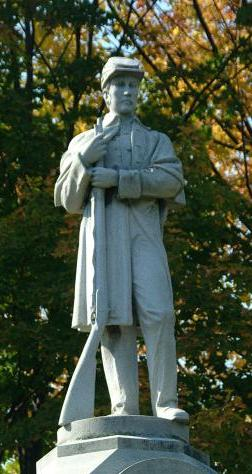
\includegraphics[width=0.3\linewidth]{images/SCP.011.jpg}
    \caption*{SCP-011}
\end{figure}

\bb{项目编号:}SCP-011

\bb{项目等级:}Safe

\bb{特殊收容措施:}SCP-011和其周围的场地需要每天清理一次。安全上建议,清理应该在日落至少30分钟后开始。清理工作必须至少有2个人员进行,要求必须能够注意到目标的异常动静和残渣的清理。如果因为什么意外导致目标有2天以上没有清理,当地居民必须被指示不得靠近目标。

[收容程序2004年作废]

\bb{描述:}SCP-011是一个位于佛蒙特州伍德斯托克的美国内战纪念雕像。雕像的外形是一个手扶滑膛枪于身侧的年轻士兵形象,场地内散布着一些花岗岩残渣。偶尔,SCP-011被目击使用滑膛枪向那些试图在雕像身上降落和排泄的鸟类射击。报告显示雕像移动时发出花岗岩摩擦声但是没有导致任何结构损坏。奇怪的是,枪击发出的声音和普通枪支没有任何区别,尽管目击者指出雕像只使用花岗岩子弹和花岗岩火药装填滑膛枪(而没有妨碍滑膛枪击发)。尽管有此类举动,一些鸟粪还是“攻击”了SCP-011,报告显示当雕像被很多鸟粪覆盖的时候表情很苦恼,在非常偶然的情况下雕像会射击人类。

\bb{附录:}被指定维护SCP-011的人员必须阅读\#011-1维护摘要。

\bb{文件\#011-1:维护摘要}

[文件记录2004-指定人员安全等级2\slash011或者以上]

附加信息:SCP-011的自从1995年第一次记录后越来越频繁。在2004年,雕像的收容措施被撤销但是仍旧处于目视监视下。下面的档案记录了关于雕像活动的主要事件。

\begin{scpbox}

时间表:\\
3.12.1995-伍德斯托克居民报告雕像的眼睛在转动,第一次记录\\
9.30.1995-雕像第一次击发滑膛枪\\
10.9.1995-雕像开始射击天上的鸟类\\
1.25.1996-编级为SCP-011,开始收容措施\\
4.14.1997-雕像被目击到偶然移动和张望四周\\
5.3.2000-在管理员████ ████████ 开玩笑得对SCP-011说“射得好!”,雕像用非常纯正的人类嗓音回应道“谢谢”,雕像第一次说话\\
10.22.2001-SCP-011开始和管理员 █████████ █████交流\\
2001-停止射击鸟类\\
2.6.2002-在 █████████ █████的恳求下,SCP-011走下了底座\\
2003-2004-SCP-011的自我意识达到了人类等级\\
11.10.2004-收容措施撤销,监护权移交给█████████ █████\\
5.17.2005-█████████ █████报告SCP-011被她所吸引\\
8.29.2006-最近更多的智力测试显示其智商达到133

\end{scpbox}

